%%%%(c)
%%%%(c)  This file is a portion of the source for the textbook
%%%%(c)
%%%%(c)    Abstract Algebra: Theory and Applications
%%%%(c)    Copyright 1997 by Thomas W. Judson
%%%%(c)
%%%%(c)  See the file COPYING.txt for copying conditions
%%%%(c)
%%%%(c)
\chap{Algebraic Coding Theory}{algcodes}
 

Coding theory is an application of algebra that has become
increasingly important over the last several decades. When we transmit
data, we are concerned about sending a message over a channel that
could be affected by ``noise.'' We wish to be able to encode and
decode the information in a manner that will allow the detection, and
possibly the correction, of errors caused by noise. This situation
arises in many areas of communications, including radio, telephone,
television, computer communications, and even compact disc player
technology. Probability, combinatorics, group theory, linear algebra,
and polynomial rings over finite fields all play important roles in
coding theory.  
 

\section{Error-Detecting and Correcting Codes}

Let us examine a simple model of a communications system for
transmitting and receiving coded messages (Figure~\ref{encoding}).  

\begin{figure}[htb] %Replaced figure with tikz figure - TWJ 5/10/2010
\begin{center}
\tikzpreface{algcode_encode_decode}
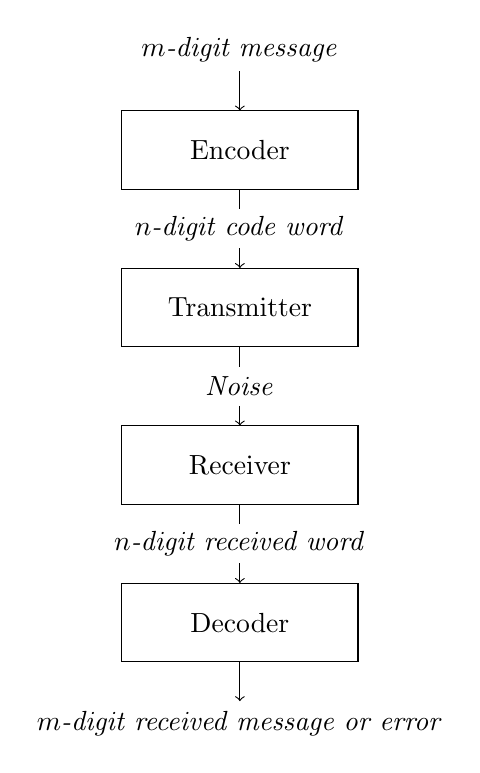
\begin{tikzpicture}[scale=1]

\draw [->] (0,8)  node [above] {\emph{$m$-digit message}} -- (0,7.5);

\node at (0,7) {Encoder};
\draw (-1.5,6.5) rectangle (1.5,7.5);
\draw (0,6.5)  -- (0,6.25);
\draw [->] (0,5.75)  -- (0,5.5);
\node at (0,6) {\emph{$n$-digit code word}};

\node at (0,5) {Transmitter};
\draw (-1.5,4.5) rectangle (1.5,5.5);
\draw (0,4.5)  -- (0,4.25);
\draw [->] (0,3.75)  -- (0,3.5);
\node at (0,4) {\emph{Noise}};

\node at (0,3) {Receiver};
\draw (-1.5,2.5) rectangle (1.5,3.5);
\draw (0,2.5)  -- (0,2.25);
\draw [->] (0,1.75)  -- (0,1.5);
\node at (0,2) {\emph{$n$-digit received word}};

\node at (0,1) {Decoder};
\draw (-1.5,0.5) rectangle (1.5,1.5);
\draw [->] (0,0.5)  -- (0,0) node [below] {\emph{$m$-digit received message or error}};

\end{tikzpicture}

\caption{Encoding and decoding messages}
\end{center}
\label{encoding}
\end{figure}

Uncoded messages may be composed of letters or characters, but
typically they consist of binary $m$-tuples. These messages are
encoded into codewords, consisting of binary $n$-tuples, by a device
called an \boldemph{encoder}. The message is transmitted and then decoded.
We will consider the occurrence of errors during transmission. An
\boldemph{error} occurs if there is a change in one or more bits in the
codeword. A \boldemph{decoding scheme} is a method that either converts
an arbitrarily received $n$-tuple into a meaningful decoded message or
gives an error message for that $n$-tuple. If the received message is
a codeword (one of the special $n$-tuples allowed to be transmitted),
then the decoded message must be the unique message that was encoded
into the codeword. For received non-codewords, the decoding scheme will
give an error indication, or, if we are more clever, will actually try
to correct the error and reconstruct the original message. Our goal is
to transmit error-free messages as cheaply and quickly as possible.
 
 
\begin{example}{repeat}
One possible coding scheme would be to send a message several
times and to compare the received copies with one another. Suppose
that the message to be encoded is a binary $n$-tuple $(x_{1}, x_{2},
\ldots, x_{n})$. The message is encoded into a binary $3n$-tuple by
simply repeating the message three times: 
\[
(x_{1}, x_{2}, \ldots, x_{n})
\mapsto
(x_{1}, x_{2}, \ldots, x_{n}, x_{1}, x_{2}, \ldots, x_{n},
x_{1}, x_{2}, \ldots, x_{n}).
\]
To decode the message, we choose as the $i$th digit the one that
appears in the $i$th place in at least two of the three transmissions.
For example, if the original message is $(0110)$, then the transmitted
message will be \mbox{$(0110\;  0110\;  0110)$}. If there is a transmission error
in the fifth digit, then the received codeword will be
$(0110\;  1110\;  0110)$, which will be correctly decoded as
$(0110)$.\footnote{We will adopt the convention that bits are numbered
left to right in binary $n$-tuples.} 
This triple-repetition method will automatically detect and correct
all single errors, but it is slow and inefficient: to send a message
consisting of $n$ bits, $2n$ extra bits are required, and we can only
detect and correct single errors. We will see that it is possible to
find an encoding scheme that will encode a message of $n$ bits into
$m$ bits with $m$ much smaller than $3n$.
\end{example}
 
 
\begin{example}{even_parity}
\boldemph{Even parity}, a  commonly  used coding scheme, is much
more efficient than the simple repetition scheme. The ASCII (American
Standard Code for Information Interchange) coding system uses binary
8-tuples, yielding $2^{8} = 256$ possible 8-tuples. However, only seven
bits are needed since there are only $2^7 = 128$ ASCII characters.
What can or should be done with the extra bit? Using the full eight
bits, we can detect single transmission errors. For example, the ASCII
codes for A, B, and C are 
\begin{align*}
\mbox{A} & = 65_{10} = 01000001_{2}, \\
\mbox{B} & = 66_{10} = 01000010_{2}, \\
\mbox{C} & = 67_{10} = 01000011_{2}.
\end{align*}
Notice that the leftmost bit is always set to 0; that is, the 128 ASCII
characters have codes 
\begin{align*}
00000000_{2} & = 0_{10}, \\
& \vdots \\
01111111_{2} & = 127_{10}.
\end{align*}
The bit can be used for error checking on the other seven bits. It is
set to either 0 or 1 so that the total number of 1 bits in the
representation of a character is even. Using even parity, the codes
for A, B, and C now become 
\begin{align*}
\mbox{A} & = 01000001_{2}, \\
\mbox{B} & = 01000010_{2}, \\
\mbox{C} & = 11000011_{2}.
\end{align*}
Suppose an A is sent and a transmission error in the sixth
bit is caused by noise over the communication channel so that 
(0100\; 0101) is received. We know an error has occurred since the
received word has an odd number of 1's, and we can now request that the
codeword be transmitted again. When used for error checking, the
leftmost bit is called a \boldemph{parity check bit}.  
 
 
By far the most common error-detecting
codes used in computers are based on the addition of a parity bit.
Typically, a computer stores information in $m$-tuples called \boldemph{
words}. Common word lengths are 8, 16, and 32 bits. One bit in the 
word is set aside as the parity check bit, and is not used to store
information. This bit is set to either 0 or 1, depending on the
number of 1's in the word. 
 
 
Adding a parity check bit allows the detection of all single errors
because changing a single bit either increases or decreases the number
of 1's by one, and in either case the parity has been changed from
even to odd, so the new word is not a codeword. (We could also
construct an error detection scheme based on \boldemph{odd parity}; that
is, we could set the parity check bit so that a codeword always has an
odd number of 1's.)  
\end{example}
 
 
The even parity system is easy to implement, but has two drawbacks.
First, multiple errors are not detectable. Suppose an A is sent and 
the first and seventh bits are changed from 0 to 1. The received word
is a codeword, but will be decoded into a C instead of an A.
Second, we do not have the ability to correct errors.  If the 8-tuple
(1001\; 1000) is received, we know that an error has occurred, but we
have no idea which bit has been changed. We will now investigate a
coding scheme that will not only allow us to detect transmission
errors but will actually correct the errors. 

 
 
\begin{table}[htb]\label{repetition_code}
\begin{center}{\small
\begin{tabular}{|lc|cccccccc|}
\hline
& & \multicolumn{8}{|c|}{Received Word}    \\
            &     & 000 & 001 & 010 & 011 & 100 & 101 & 110
& 111 \\ \hline
Transmitted & 000 & 0   & 1   & 1   & 2   & 1   & 2   & 2
& 3 \\
Codeword   & 111 & 3   &  2  & 2   &  1  &  2  &   1 &  1
&  0 \\ \hline
\end{tabular}
}
\caption{A repetition code}
\end{center}
\end{table}

 
\begin{example}{nearest}
Suppose that our original message is either a 0 or a 1, and that 0
encodes to (000) and 1 encodes to (111). If only a single
error occurs during transmission, we can detect and correct the
error. For example, if a 101 is received, then the second bit must
have been changed from a 1 to a 0.  The originally transmitted
codeword must have been (111). 	This method will detect and correct 
all single errors. 
 
 
In Table~\ref{repetition_code}, we present all possible words that might be received
for the transmitted codewords (000) and (111). Table~\ref{repetition_code} also shows 
the number of bits by which each received 3-tuple differs from each
original codeword. 
\end{example}
 
 
 
\subsection*{Maximum-Likelihood Decoding}

%% Footnote in subsection header undigestable by tex4ht
%%   it can follow just outside the {},
%%   but formats weirdly in both PDF and XHTML
%% \footnote{This section
%% requires a knowledge of probability, but can be
%% skipped without loss of continuity.}

%Label repaired.  Suggested by R. Beezer.
%TWJ - 12/19/2011
The coding scheme presented in Example~\ref{example:algcodes:nearest} is not a complete solution to
the problem because it does not account for the possibility of
multiple errors. For example, either a (000) or a (111) could be sent
and a (001) received. We have no means of deciding from the received
word whether there was a single error in the third bit or two errors,
one in the first bit and one in the second.  No matter what coding 
scheme is used, an incorrect message could
be received: we could transmit a (000), have errors in all three
bits, and receive the codeword (111). It is important to make explicit
assumptions about the likelihood and distribution of transmission
errors so that, in a particular application, it will be known whether
a given
error detection scheme is appropriate. We will assume that
transmission errors are rare, and, that when they do occur, they occur
independently in each bit; that is, if $p$ is the probability of an
error in one bit and $q$ is the probability of an error in a different
bit, then the probability of errors occurring in both of these bits at
the same time is $pq$. We will also assume that a received $n$-tuple 
is
decoded into a codeword that is closest to it; that is, we assume that
the receiver uses \boldemph{maximum-likelihood
decoding}\index{Maximum-likelihood decoding}.
 
 
\begin{figure}[htb]  %Replaced figure with tikz figure - TWJ 5/10/2010
\begin{center}
\tikzpreface{algcode_binary_channel}
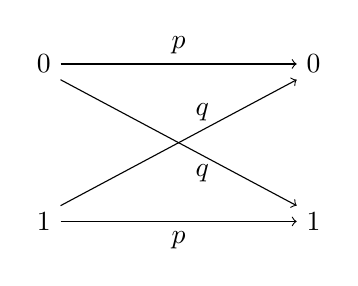
\begin{tikzpicture}[scale=1]

\node at (1.5,0) [below] {$p$};
\draw [->] (0,0)  node [left] {1} -- (3,0) node [right] {1};
\node at (1.5,2) [above] {$p$};
\draw [->] (0,2)  node [left] {0} -- (3,2) node [right] {0};

\draw [->] (0,0.2) -- (3,1.8);
\draw [->] (0,1.8) -- (3,0.2);

\node at (1.8,1.15) [above] {$q$};
\node at (1.8,0.85) [below] {$q$};


\end{tikzpicture}

\end{center}
\caption{Binary symmetric channel}
\label{channel}
\end{figure}
 
 
 
A \boldemph{binary symmetric channel}\index{Binary symmetric channel}
is a model that consists of a transmitter capable of sending a binary 
signal, either a 0 or a 1, together with a receiver. Let $p$ be the 
probability that the signal is correctly
received. Then $q=1-p$ is the probability of an incorrect reception.
If a 1 is sent, then the probability that a 1 is received is $p$ and
the probability that a 0 is received is $q$ (Figure~\ref{channel}).
The probability that no errors occur during the transmission of a binary
codeword of length $n$ is $p^{n}$. For example, if $p=0.999$ and a
message consisting of 10,000 bits is sent, then the probability of a
perfect transmission is 
\[
(0.999)^{10,000} \approx 0.00005.
\]
 
 
\begin{theorem}
If a binary $n$-tuple $(x_{1}, \ldots, x_{n})$ is transmitted across a
binary symmetric channel with probability $p$ that no error will occur
in each coordinate, then the probability that there are errors in
exactly $k$ coordinates~is
\[
\binom{n}{k} q^kp^{n-k}.
\]
\end{theorem}
 
 
\begin{proof}
Fix $k$ different coordinates. We first compute the probability that
an error has occurred in this fixed set of coordinates. The
probability of an error occurring in a particular one of these $k$
coordinates is $q$; the probability that an error will not occur
in any of the remaining $n-k$ coordinates is $p$. The
probability of each of these $n$ independent events is
$q^{k}p^{n-k}$. The number of possible error patterns with exactly $k$
errors occurring is equal to 
\[
\binom{n}{k} 
= \frac{n!}{k!(n-k)!},
\]
the number of combinations of $n$ things taken $k$ at a time. Each of
these error patterns has probability $q^{k}p^{n-k}$ of occurring;
hence, the probability of all of these error patterns is
\[
\binom{n}{k} 
q^{k}p^{n-k}.
\]
\end{proof}
 
 
\begin{example}{probability}
Suppose that $p = 0.995$ and a 500-bit message is sent. The
probability that the message was sent error-free is 
\[
p^{n} = (0.995)^{500} \approx 0.082.
\]
The probability of exactly one error occurring is
\[
\binom{n}{1} 
qp^{n-1}= 500(0.005)(0.995)^{499}
\approx 0.204.
\]
The probability of exactly two errors is
\[
\binom{n}{2} 
q^{2}p^{n-2}=
\frac{500 \cdot 499}{2}(0.005)^{2}(0.995)^{498} \approx
0.257.
\]
The probability of more than two errors is approximately
\[
1-0.082-0.204 -0.257=0.457.
\]
\end{example}
 
 
\subsection*{Block Codes}
 
 
If we are to develop efficient error-detecting and error-correcting
codes, we will need more sophisticated mathematical tools.  Group
theory  will allow faster methods of encoding and decoding messages. A
code is an $(n, m)$-\boldemph{block code} if the information that is to be
coded can be divided into blocks of $m$ binary digits, each of which
can be encoded into $n$ binary digits. More specifically, an $(n,
m)$-block code consists of an \boldemph{encoding function} 
\[
E:{\mathbb Z}^{m}_{2} \rightarrow {\mathbb Z}^{n}_{2}
\]
and a \boldemph{decoding function}
\[
D:{\mathbb Z}^{n}_{2} \rightarrow {\mathbb Z}^{m}_{2}.
\]
A \boldemph{codeword} is any element in the image of $E$. We also require
that $E$ be one-to-one so that two information blocks will not be
encoded into the same codeword. If our code is to be error-correcting,
then $D$ must be onto.
 
 
\begin{example}{BlockCode}
The even-parity coding system developed to detect single errors in
ASCII characters is an $(8,7)$-block code. The encoding function is
\[
E(x_7, x_6, \ldots, x_1) = (x_8, x_7,  \ldots, x_1),
\]
where $x_8 = x_7 + x_6 + \cdots + x_1$ with addition in ${\mathbb Z}_2$. 
\end{example}
 

 
Let ${\mathbf x} = (x_1, \ldots, x_n)$ and ${\mathbf y} = (y_1, \ldots,
y_n)$ be binary $n$-tuples. The \boldemph{Hamming distance}\index{Hamming
distance} or \boldemph{distance}, $d({\mathbf x}, {\mathbf
y})$\label{noteHammingdist}, between ${\mathbf x}$ and ${\mathbf y}$ is
the number of bits in which ${\mathbf x}$ and ${\mathbf y}$ differ. The
distance between two codewords is the minimum number of transmission
errors required to change one codeword into the other. The
\boldemph{minimum distance}\index{Code!minimum distance of} for a code,
$d_{\min}$\label{notemindist}, is the minimum of all distances
$d({\mathbf x}, {\mathbf y})$, where ${\mathbf x}$ and ${\mathbf y}$ are
distinct codewords. The \boldemph{weight}\index{Weight of a codeword},
$w({\mathbf x})$\label{noteweight}, of a binary codeword ${\mathbf x}$ is
the number of 1's in ${\mathbf x}$. Clearly, $w({\mathbf x}) = d({\mathbf
x}, {\mathbf 0})$, where ${\mathbf 0} = (00 \cdots 0)$. 
 
 
\begin{example}{min_distance}
Let ${\mathbf x} = (10101)$, ${\mathbf y} = (11010)$, and ${\mathbf z} =
(00011)$ be all of the codewords in some code $C$. Then we have the
following Hamming distances: 
\[
d({\mathbf x},{\mathbf y}) = 4, \qquad
d({\mathbf x},{\mathbf z}) = 3, \qquad
d({\mathbf y},{\mathbf z}) = 3.
\]
The minimum distance  for this code is 3. We also have the
following weights: 
\[
w({\mathbf x}) = 3, \qquad
w({\mathbf y}) = 3, \qquad
w({\mathbf z}) = 2.
\]
\end{example}
 
 
The following proposition lists some basic properties about the weight
of a codeword and the distance between two codewords. The proof is
left as an exercise.
 
 
\begin{proposition}
Let ${\mathbf x}$, ${\mathbf y}$, and ${\mathbf z}$ be binary $n$-tuples.
Then 
\begin{enumerate}
 
\rm \item \it
$w({\mathbf x}) = d( {\mathbf x}, {\mathbf 0})$; 
 
\rm \item \it
$d( {\mathbf x}, {\mathbf y}) \geq 0$; 
 
\rm \item \it
$d( {\mathbf x}, {\mathbf y}) = 0$ exactly when ${\mathbf x} = {\mathbf y}$; 
 
\rm \item \it
$d( {\mathbf x}, {\mathbf y})= d( {\mathbf y}, {\mathbf x})$; 
 
\rm \item \it
$d( {\mathbf x}, {\mathbf y}) \leq d( {\mathbf x}, {\mathbf z}) + d( {\mathbf
z}, {\mathbf y})$. 
 
\end{enumerate}
\end{proposition}
 
 
The weights in a particular code are usually much easier to compute
than the Hamming distances between all codewords in the code. If a
code is set up carefully, we can use this fact to our advantage.
 
 
Suppose that ${\mathbf x} = (1101)$ and ${\mathbf y} = (1100)$ are
codewords in some code. If we transmit (1101) and an error occurs in
the rightmost bit, then (1100) will be received. Since (1100) is a
codeword, the decoder will decode (1100) as the transmitted message.
This code is clearly not very appropriate for error detection. The
problem is that $d({\mathbf x}, {\mathbf y}) = 1$. If ${\mathbf x} = (1100)$
and ${\mathbf y} = (1010)$ are codewords, then $d({\mathbf x}, {\mathbf y})
= 2$. If ${\mathbf x}$ is transmitted and a single error occurs, then
${\mathbf y}$ can never be received. Table~\ref{4-bit_words} gives the distances
between all 4-bit codewords in which the first three bits carry
information and the fourth is an even parity check bit. We can see
that the minimum distance here is 2; hence, the code is suitable as
a single error-correcting code. 
 
 
\begin{table}[hbt]
{\small
\begin{center}
\begin{tabular}{|c|cccccccc|}
\hline
    & 0000 & 0011 & 0101 & 0110 & 1001 & 1010 & 1100 & 1111
\\ \hline
0000 & 0 & 2 & 2 & 2 & 2 & 2 & 2 & 4 \\
0011 & 2 & 0 & 2 & 2 & 2 & 2 & 4 & 2 \\
0101 & 2 & 2 & 0 & 2 & 2 & 4 & 2 & 2 \\
0110 & 2 & 2 & 2 & 0 & 4 & 2 & 2 & 2 \\
1001 & 2 & 2 & 2 & 4 & 0 & 2 & 2 & 2 \\
1010 & 2 & 2 & 4 & 2 & 2 & 0 & 2 & 2 \\
1100 & 2 & 4 & 2 & 2 & 2 & 2 & 0 & 2 \\
1111 & 4 & 2 & 2 & 2 & 2 & 2 & 2 & 0 \\
\hline
\end{tabular}
\caption{Distances between 4-bit codewords}\label{4-bit_words}
\end{center}
}
\end{table}
 
 
 
To determine exactly what the error-detecting and error-correcting
capabilities for a code are, we need to analyze the minimum distance
for the code. Let ${\mathbf x}$ and ${\mathbf y}$ be codewords. If
$d({\mathbf x}, {\mathbf y}) = 1$ and an error occurs where ${\mathbf x}$
and ${\mathbf y}$ differ, then ${\mathbf x}$ is changed to ${\mathbf y}$.
The received codeword is ${\mathbf y}$ and no error message is given.
Now suppose $d({\mathbf x}, {\mathbf y}) = 2$. Then a single error cannot
change ${\mathbf x}$ to ${\mathbf y}$. Therefore, if $d_{\min} = 2$, we
have the ability to detect single errors. However, suppose that
$d({\mathbf x}, {\mathbf y}) = 2$, ${\mathbf y}$ is sent, and a noncodeword
${\mathbf z}$ is received such that
\[
d({\mathbf x}, {\mathbf z}) = d({\mathbf y}, {\mathbf z}) = 1.
\]
Then the decoder cannot decide between ${\mathbf x}$ and ${\mathbf y}$. Even
though we are aware that an error has occurred, we do not know what
the error is.
 
 
Suppose $d_{\min} \geq 3$. Then the maximum-likelihood decoding scheme
corrects all single errors. Starting with a codeword ${\mathbf x}$, an
error in the transmission of a single bit gives ${\mathbf y}$ with
$d({\mathbf x}, {\mathbf y}) = 1$, but $d({\mathbf z}, {\mathbf y}) \geq 2$
for any other codeword ${\mathbf z} \neq {\mathbf x}$. If we do not
require the correction of errors, then we can detect multiple errors
when a code has a minimum distance that is greater than 3.  
 
 
\begin{theorem}\label{algecodes:min_distance_theorem}
Let $C$ be a code with $d_{\min} = 2n + 1$. Then $C$ can correct any
$n$ or fewer errors.  Furthermore, any $2n$ or fewer errors can be
detected in~$C$. 
\end{theorem}
 
 
\begin{proof}
Suppose that a codeword ${\mathbf x}$ is sent and the word ${\mathbf y}$
is received with at most $n$ errors. Then $d( {\mathbf x}, {\mathbf y})
\leq n$. If ${\mathbf z}$ is any codeword other than ${\mathbf x}$, then
\[
2n+1
\leq
d( {\mathbf x}, {\mathbf z})
\leq
d( {\mathbf x}, {\mathbf y}) + d( {\mathbf y}, {\mathbf z})
\leq
n + d( {\mathbf y}, {\mathbf z}).
\]
Hence, $d({\mathbf y}, {\mathbf z} ) \geq n+1$ and ${\mathbf y}$ will be
correctly decoded as ${\mathbf x}$. Now suppose that ${\mathbf x}$ is
transmitted and ${\mathbf y}$ is received and that at least one error 
has occurred, but not more than $2n$ errors. Then $1 \leq d( {\mathbf x},
{\mathbf y} ) \leq 2n$.  Since the minimum distance between codewords is
$2n +1$, ${\mathbf y}$ cannot be a codeword.  Consequently, the code can
detect between 1 and $2n$ errors. 
\end{proof}
 
 
\begin{example}{single_correct}
In Table~\ref{Hamming_dist}, the codewords ${\mathbf c}_1 = (00000)$, ${\mathbf c}_2 = (00111)$,
${\mathbf c}_3 = (11100)$, and ${\mathbf c}_4 = (11011)$ determine a
single error-correcting code.  
\end{example}
 
 
\begin{table}[htb]

\begin{center}
{\small
\begin{tabular}{|c|cccc|}
\hline
      & 00000 & 00111 & 11100 & 11011 \\ \hline
00000 & 0     & 3     & 3     & 4 \\
00111 & 3     & 0     & 4     & 3 \\
11100 & 3     & 4     & 0     & 3 \\
11011 & 4     & 3     & 3     & 0 \\
\hline
\end{tabular}
}
\caption{ Hamming distances for an error-correcting code}\label{Hamming_dist}
\end{center}
\end{table}
 
 
 
 
 
\histhead
 
 
\noindent{\small \histf
Modern coding theory began in 1948 with C. Shannon's\index{Shannon,
C.} paper, ``A Mathematical Theory of Information'' [7]. This paper offered
an example of an algebraic code, and Shannon's Theorem proclaimed
exactly how good codes could be expected to be. Richard
Hamming\index{Hamming, R.} began working with linear codes at Bell
Labs in the late 1940s and early 1950s after becoming frustrated
because the programs that he was running could not recover from simple
errors generated by noise. Coding theory has grown tremendously in the
past several years. \textit{The Theory of Error-Correcting Codes}, by 
MacWilliams and Sloane [5], published in 1977, already
contained over 1500 references. Linear codes (Reed-Muller $(32,
6)$-block codes) were used on NASA's Mariner space probes.  More recent
space probes such as Voyager have used what are called convolution
codes.  Currently, very active research is being done with Goppa
codes, which are heavily dependent on algebraic geometry.
\histbox
} 
 
 
\section{Linear Codes}
 
 
To gain more knowledge of a particular code and develop more efficient
techniques of encoding, decoding, and error detection, we need to add
additional structure to our codes. One way to accomplish this is to
require that the code also be a group. A \boldemph{group
code}\index{Code!group} is a code that is also a subgroup of ${\mathbb
Z}_2^n$.  
 
 
To check that a code is a group code, we need only verify one thing.
If we add any two elements in the code, the result must be an $n$-tuple
that is again in the code. It is not necessary to check that the
inverse of the $n$-tuple is in the code, since every codeword is its own
inverse, nor is it necessary to check that ${\mathbf 0}$ is a codeword.
For instance,
\[
(11000101) + (11000101) = (00000000).
\]
 
 
\begin{example}{weights}
Suppose that we have a code that consists of the following 7-tuples: 
\[
\begin{array}{cccc}
(0000000) & (0001111) & (0010101) & (0011010) \\
(0100110) & (0101001) & (0110011) & (0111100) \\
(1000011) & (1001100) & (1010110) & (1011001) \\
(1100101) & (1101010) & (1110000) & (1111111).
\end{array}
\]
It is a straightforward though tedious task to verify that this code
is also a subgroup of ${\mathbb Z}_2^7$ and, therefore, a group code.
This code is a single error-detecting and single error-correcting 
code, but
it is a long and tedious process to compute all of the distances
between  pairs of codewords to determine that $d_{\min} = 3$. It is
much easier to see that the minimum weight of all the nonzero
codewords is 3. As we will soon see, this is no coincidence.
However, the relationship between weights and distances in a
particular code is heavily dependent on the fact that the code is a
group. 
\end{example}
 
 
\begin{lemma}
Let ${\mathbf x}$ and ${\mathbf y}$ be  binary $n$-tuples. Then $w({\mathbf
x} + {\mathbf y}) = d({\mathbf x}, {\mathbf y})$. 
\end{lemma}
 
 
\begin{proof}
Suppose that ${\mathbf x}$ and ${\mathbf y}$ are binary $n$-tuples. Then
the distance between ${\mathbf x}$ and ${\mathbf y}$ is exactly the number
of places in which ${\mathbf x}$ and ${\mathbf y}$ differ. But ${\mathbf x}$
and ${\mathbf y}$ differ in a particular coordinate exactly when the sum
in the coordinate is 1, since
\begin{align*}
1 + 1 & = 0 \\
0 + 0 & = 0 \\
1 + 0 & = 1 \\
0 + 1 & = 1.
\end{align*}
Consequently, the weight of the sum must be the distance between the two
codewords.
\end{proof}
 
 
\begin{theorem}
Let $d_{\min}$ be the minimum distance for a group code $C$. Then
$d_{\min}$ is the minimum of all the nonzero weights of the nonzero
codewords in $C$. That is, 
\[
d_{\min} = \min\{ w({\mathbf x}) : { {\mathbf x} \neq {\mathbf 0} } \}.
\]
\end{theorem}
 
 
\begin{proof}
Observe that
\begin{align*}
d_{\min} & =  \min \{ d({\mathbf x},{\mathbf y}) : {\mathbf x}
\neq
{\mathbf y} \} \\
&=  \min \{ d({\mathbf x},{\mathbf y}) : {\mathbf x}+{\mathbf y}
\neq {\mathbf 0} \} \\
&= \min\{ w({\mathbf x} + {\mathbf y}) : {\mathbf x}+{\mathbf y}
\neq {\mathbf 0} \} \\
& =  \min\{ w({\mathbf z}) : {\mathbf z} \neq {\mathbf 0} \}.
\end{align*}
\end{proof}
 
 
\subsection*{Linear Codes}
 
 
From Example~\ref{example:algcodes:weights}, it is now easy to check that the minimum nonzero
weight is 3; hence, the code does indeed detect and correct all
single errors. We have now reduced the problem of finding ``good''
codes to that of generating group codes. One easy way to generate
group codes is to employ a bit of matrix theory. 
 
 
Define the \boldemph{inner product}\index{Inner product} of two binary
$n$-tuples to be 
\[
{\mathbf x} \cdot {\mathbf y} = x_1 y_1 + \cdots + x_n y_n,
\]
where ${\mathbf x} = (x_1, x_2, \ldots, x_n)^{\rm t}$ and ${\mathbf y} =
(y_1, y_2, \ldots, y_n)^{\rm t}$ are column vectors.\footnote{Since we
will be working with matrices, we will write binary $n$-tuples as
column vectors for the remainder of this chapter.} For example, if
${\mathbf x} = (011001)^{\rm t}$ and ${\mathbf y} = (110101)^{\rm t}$,
then ${\mathbf x} \cdot {\mathbf y} = 0$. We can also look at an inner
product as the product of a row matrix with a column matrix; that is, 
\begin{align*}
{\mathbf x} \cdot {\mathbf y} & = {\mathbf x}^{\rm t}  {\mathbf y}
\\
& =
\begin{pmatrix}
x_1 & x_2 & \cdots & x_n
\end{pmatrix}
\begin{pmatrix}
y_1 \\
y_2 \\
\vdots \\
y_n
\end{pmatrix} \\
& =
x_{1}y_{1} + x_{2}y_{2} + \cdots + x_{n}y_{n}.
\end{align*}
 
 
\begin{example}{matrix_codes}
Suppose that the words to be encoded consist of all binary
\mbox{3-tuples}
and that our encoding scheme is even-parity. To encode an arbitrary
3-tuple, we add a fourth bit to obtain an even number of 1's. Notice
that an arbitrary $n$-tuple ${\mathbf x} = (x_1, x_2, \ldots, x_n)^{\rm
t}$ has an even number of 1's exactly when $x_1 + x_2 + \cdots + x_n =
0$; hence, a 4-tuple ${\mathbf x} = (x_1, x_2, x_3, x_4)^{\rm t}$ has an
even number of 1's if $ x_1+ x_2+ x_3+ x_4 = 0$, or 
\[
{\mathbf x} \cdot {\mathbf 1} 
= 
{\mathbf x}^{\rm t} {\mathbf 1} 
=
\begin{pmatrix}
x_1 & x_2 & x_3 & x_4
\end{pmatrix}
\begin{pmatrix}
1 \\ 1 \\ 1 \\ 1
\end{pmatrix} = 0.
\]
This example leads us to hope that there is a connection between
matrices and coding theory. 
\end{example}
 
 
Let ${\mathbb M}_{m \times n}({\mathbb Z}_2)$\label{notembyn} denote the set
of all $m \times n$ matrices with entries in ${\mathbb Z}_2$. We do
matrix operations as usual except that all our addition and multiplication
operations occur in ${\mathbb Z}_2$. Define the \boldemph{null
space}\index{Matrix!null space of}\index{Null space!of a matrix} of 
a matrix $H \in {\mathbb M}_{m \times n}({\mathbb Z}_2)$ to be the set of
all binary $n$-tuples ${\mathbf x}$ such that $H{\mathbf x} = {\mathbf 0}$.
We denote the null space of a matrix $H$ by ${\rm Null}(H)$\label{notenull}.  
 
 
\begin{example}{group_code}
Suppose that
\[
H =
\begin{pmatrix}
0 & 1 & 0 & 1 & 0 \\
1 & 1 & 1 & 1 & 0 \\
0 & 0 & 1 & 1 & 1
\end{pmatrix}.
\]
For a 5-tuple ${\mathbf x} = (x_1, x_2, x_3, x_4, x_5)^{\rm t}$ to be in
the null space of $H$, $H{\mathbf x} = {\mathbf 0}$. Equivalently, the
following system of equations must be satisfied:   
\begin{align*}
  x_2 +  x_4  & =  0 \\
x_1 +  x_2 + x_3  + x_4   & =  0 \\
  x_3  + x_4  +  x_5 & =  0.
\end{align*}
The set of binary 5-tuples satisfying these equations is
\[
(00000) \qquad (11110) \qquad (10101) \qquad (01011).
\]
This code is easily determined to be a group code.
\end{example}
 
 
\begin{theorem}
Let $H$ be in ${\mathbb M}_{m \times n}({\mathbb Z}_2)$. Then the null space of
$H$ is a group~code. 
\end{theorem}
 
 
\begin{proof}
Since each element of ${\mathbb Z}_2^n$ is its own inverse, the only
thing that really needs to be checked here is closure. Let ${\mathbf x},
{\mathbf y} \in {\rm Null}(H)$ for some matrix $H$ in ${\mathbb M}_{m \times
n}({\mathbb Z}_2)$. Then $H{\mathbf x} = {\mathbf 0}$ and $H{\mathbf y} =
{\mathbf 0}$. So 
\[
H({\mathbf x}+{\mathbf y}) 
=
H{\mathbf x} + H{\mathbf y} = {\mathbf 0}
+
{\mathbf 0}
= {\mathbf 0}.
\]
Hence, ${\mathbf x}+{\mathbf y}$ is in the null space of $H$ and
therefore must be a codeword. 
\hspace*{1in}
\end{proof}
 
%typo correction.  Suggested by J. Buller.
%TWJ - 12/20/2011

\medskip
 
 
A code is a \boldemph{linear code}\index{Code!linear} if it is
determined by the null space of some matrix $H \in {\mathbb M}_{m \times
n}({\mathbb Z}_2)$.  
 
 
 
\begin{example}{linear_code}
Let $C$ be the code given by the matrix
\[
H =
\begin{pmatrix}
0 & 0 & 0 & 1 & 1 & 1 \\
0 & 1 & 1 & 0 & 1 & 1 \\
1 & 0 & 1 & 0 & 0 & 1
\end{pmatrix}.
\]
Suppose that the 6-tuple ${\mathbf x} = (010011)^{\rm t}$ is received.
It is a simple matter of matrix multiplication to determine whether or
not ${\mathbf x}$ is a codeword. Since 
\[
H{\mathbf x} =
\begin{pmatrix} 
0 \\ 1 \\ 1
\end{pmatrix},
\]
the received word is not a codeword.  We must either attempt to
correct the word or request that it be transmitted again.
\end{example}

%typo correction.  Suggested by J. Buller.
%TWJ - 12/20/2011
 
 
 
\section{Parity-Check and Generator Matrices}
 
 
We need to find a systematic way of generating linear codes as well as
fast methods of decoding. By examining the properties of a matrix $H$
and by carefully choosing $H$, it is possible to develop very
efficient methods of encoding and decoding messages. To this end, we 
will introduce standard generator and canonical parity-check
matrices.
 
 
Suppose that $H$ is an $m \times n$ matrix with entries in
${\mathbb Z}_2$ and $n > m$. If the last $m$ columns of the
matrix form the $m \times m$ identity matrix, $I_m$, then
the matrix is a \boldemph{canonical parity-check
matrix}\index{Matrix!parity-check}. More specifically, $H= (A \mid I_m
)$, where $A$ is the $m \times (n-m)$ matrix
\[
\begin{pmatrix}
a_{11} & a_{12} & \cdots & a_{1,n-m} \\
a_{21} & a_{22} & \cdots & a_{2,n-m} \\
\vdots & \vdots \ddots & \vdots    \\
a_{m1} & a_{m2} & \cdots & a_{m,n-m}
\end{pmatrix}
\]
and $I_m$ is the $m \times m$ identity matrix
\[
\begin{pmatrix}
1 & 0 & \cdots & 0 \\
0 & 1 & \cdots & 0 \\
\vdots & \vdots \ddots & \vdots \\
0 & 0 & \cdots & 1
\end{pmatrix}.
\]
With each canonical parity-check matrix we can associate an $n \times
(n-m)$ \boldemph{standard generator matrix}\index{Matrix!generator} 
\[
G =
\left(
\frac{I_{n-m}}{A}
\right).
\]
Our goal will be to show that $G {\mathbf x} = {\mathbf y}$ if and only if
$H{\mathbf y} = {\mathbf 0}$.  Given a message block ${\mathbf x}$ to be
encoded, $G$ will allow us to quickly encode it into a linear
codeword ${\mathbf y}$. 
 
 
\begin{example}{ParityCheck}
Suppose that we have the following eight words to be
encoded:
\[
(000), (001), (010), \ldots, (111).
\]
For
\[
A =
\begin{pmatrix}
0 & 1 & 1 \\
1 & 1 & 0 \\
1 & 0 & 1
\end{pmatrix},
\]
the associated standard generator and canonical parity-check matrices
are 
\[
G=
\begin{pmatrix}
1 & 0 & 0 \\
0 & 1 & 0 \\
0 & 0 & 1 \\
0 & 1 & 1 \\
1 & 1 & 0 \\
1 & 0 & 1
\end{pmatrix}
\]
and
\[
H =
\begin{pmatrix}
0 & 1 & 1 & 1 & 0 & 0 \\
1 & 1 & 0 & 0 & 1 & 0 \\
1 & 0 & 1 & 0 & 0 & 1
\end{pmatrix},
\]
respectively.
 
 
Observe that the rows in $H$  represent the parity checks on certain
bit positions in a 6-tuple. The 1's in the identity matrix serve as
parity checks for the 1's in the same row. If ${\mathbf x} = (x_1, x_2,
x_3, x_4, x_5, x_6)$, then 
\[
{\mathbf 0}
=
H{\mathbf x}
=
\begin{pmatrix}
x_2 + x_3 + x_4 \\
x_1 + x_2 + x_5\\
x_1 + x_3 + x_6
\end{pmatrix},
\]
which yields a system of equations:
\begin{align*}
x_2 + x_3 + x_4 & = 0 \\
x_1 + x_2 + x_5 & = 0 \\
x_1 + x_3 + x_6 & = 0.
\end{align*}
Here $x_4$ serves as a check bit for $x_2$ and $x_3$; $x_5$ is a check
bit for $x_1$ and $x_2$; and $x_6$ is a check bit for $x_1$ and $x_3$.
The identity matrix keeps $x_4$, $x_5$, and $x_6$ from having to check
on each other. Hence, $x_1$, $x_2$, and $x_3$ can be arbitrary but
$x_4$, $x_5$, and $x_6$ must be chosen to ensure parity. The null
space of $H$ is easily computed to be
\[
\begin{array}{cccc}
 (000000) & (001101) & (010110) & (011011) \\
 (100011) & (101110) & (110101) & (111000).
\end{array}
\]
An even easier way to compute the null space is with the generator
matrix $G$ (Table~\ref{matrix_gen_code}). 
\end{example}
 
 
\begin{table}[htb]
{\small
\begin{center}
\begin{tabular}{|c|c|}
\hline
Message Word  & Codeword \\
${\mathbf x}$ & $G {\mathbf x}$ \\ \hline
000 & 000000 \\
001 & 001101 \\
010 & 010110 \\
011 & 011011 \\
100 & 100011 \\
101 & 101110 \\
110 & 110101 \\
111 & 111000 \\
\hline
\end{tabular}
\end{center}
}
\caption{A matrix-generated code}\label{matrix_gen_code}
\end{table}
 
 
\begin{theorem}
If $H \in {\mathbb M}_{m \times n}({\mathbb Z}_2)$ is a canonical
parity-check matrix, then ${\rm Null}(H)$ consists of all 
${\mathbf x} \in {\mathbb Z}_2^n$ whose first $n-m$ bits are arbitrary but whose last $m$ bits
are determined by $H{\mathbf x} = {\mathbf 0}$. Each of
the last $m$ bits serves as an even parity check bit for some of the
first $n-m$ bits. Hence, $H$ gives rise to an $(n, n-m)$-block code. 
\end{theorem}


 
 
We leave the proof of this theorem as an exercise. In light of the
theorem, the first $n - m$ bits in ${\mathbf x}$ are called \boldemph{
information bits} and the last $m$ bits are called \boldemph{check bits}.
In Example~\ref{example:algcodes:ParityCheck},  the first three bits are the information bits
and the last three are the check bits.
 
 
\begin{theorem}
Suppose that $G$ is an $n \times k$  standard generator matrix.  Then
$C = \left\{{\mathbf y} : G{\mathbf x} ={\mathbf y}\text{ for }{\mathbf x}\in
{\mathbb  Z}_2^k\right\}$ is an  $(n,k)$-block code. More specifically, $C$
is a group code.  
\end{theorem}
 
 
\begin{proof}
Let $G {\mathbf x}_1 = {\mathbf y}_1$ and $G {\mathbf
x}_2 ={\mathbf y}_2$ be two codewords. Then ${\mathbf y}_1
+ {\mathbf y}_2$ is in $C$ since 
\[
G( {\mathbf x}_1 + {\mathbf x}_2)
=
G {\mathbf x}_1 + G {\mathbf x}_2
=
{\mathbf y}_1 + {\mathbf y}_2.
\]
We must also show that two message blocks cannot be encoded into the
same codeword. That is, we must show that if $G {\mathbf x} = G
{\mathbf y}$, then ${\mathbf x} = {\mathbf y}$.  Suppose that $G
{\mathbf x} = G {\mathbf y}$. Then
\[
G {\mathbf x} - G {\mathbf y}
=
G( {\mathbf x} - {\mathbf y})
=
{\mathbf 0}.
\]
However, the first $k$ coordinates in $G( {\mathbf x} - {\mathbf
y})$ are exactly $x_1 -y_1, \ldots, x_k - y_k$, since they are
determined by the identity matrix, $I_k$, part of $G$. Hence, $G(
{\mathbf x} - {\mathbf y}) = {\mathbf 0}$ exactly when
${\mathbf x} = {\mathbf y}$.
\end{proof}
 
 \medskip
 
 
Before we can prove the relationship between canonical parity-check
matrices and standard generating matrices, we need to prove a lemma.
 
 
\begin{lemma}\label{ParityCheckLemma}
Let $H = (A \mid I_m )$ be an $m \times n$ canonical parity-check
matrix and $G = \left( \frac{I_{n-m} }{A} \right)$ be the
corresponding $n \times (n-m)$ standard generator matrix. Then $HG =
{\mathbf 0}$. 
\end{lemma}
 
 
\begin{proof}
Let $C = HG$.  The $ij$th entry in $C$ is
\begin{align*}
c_{ij}
& = 
\sum_{k=1}^n h_{ik} g_{kj} \\
& =  \sum_{k=1}^{n-m} h_{ik} g_{kj} + \sum_{k=n-m+1}^n h_{ik} g_{kj} \\
& = \sum_{k=1}^{n-m} a_{ik} \delta_{kj} + \sum_{k=n-m+1}^n \delta_{i-(m-n),k} a_{kj} \\
& =  a_{ij} + a_{ij} \\
& = 0,
\end{align*}
where
\[
\delta_{ij}\label{notekron}
=
\begin{cases}
1, & i = j \\
0, & i \neq j
\end{cases}
\]
is the Kronecker delta\index{Kronecker delta}.
\end{proof}
 
 
\begin{theorem}
Let $H = (A \mid I_m )$ be an $m \times n$ canonical parity-check
matrix and let $G = \left( \frac{I_{n-m} }{A} \right) $ be the $n
\times (n-m)$ standard generator matrix associated with $H$. Let $C$
be the code generated by $G$. Then ${\mathbf y}$ is in $C$ if and only
if $H {\mathbf y} = {\mathbf 0}$. In particular, $C$ is a linear code with
canonical parity-check matrix $H$. 
\end{theorem}
 
 
\begin{proof}
First suppose that ${\mathbf y} \in C$. Then $G {\mathbf x} = {\mathbf y}$
for some ${\mathbf x} \in {\mathbb Z}_2^m$. By Lemma~\ref{ParityCheckLemma}, $H {\mathbf y} = HG
{\mathbf x} = {\mathbf 0}$. 
 
 
Conversely, suppose that ${\mathbf y} = (y_1, \ldots, y_n)^{\rm t}$ is
in the null space of $H$.  We need to find an ${\mathbf x}$ in ${\mathbb
Z}_2^{n-m}$ such that $G {\mathbf x}^{\rm t} = {\mathbf y}$. Since $H
{\mathbf y} = {\mathbf 0}$, the following set of equations must be
satisfied:  
\begin{align*}
a_{11} y_1 + a_{12} y_2 + \cdots + a_{1, n-m} y_{n-m} + y_{n-m+1}
& = 0 \\
a_{21} y_1 + a_{22} y_2 + \cdots + a_{2, n-m} y_{n-m} + y_{n-m+1}
& = 0 \\
& \vdots   \\
a_{m1} y_1 + a_{m2} y_2 + \cdots + a_{m, n-m} y_{n-m} + y_{n-m+1}
& = 0.
\end{align*}
Equivalently, $y_{n-m+1}, \ldots, y_n$ are determined by $y_1, \ldots,
y_{n-m}$: 
\begin{align*}
y_{n-m+1}
& = a_{11} y_1 + a_{12} y_2 + \cdots + a_{1, n-m} y_{n-m} \\
y_{n-m+1}
& = a_{21} y_1 + a_{22} y_2 + \cdots + a_{2, n-m} y_{n-m} \\
& \vdots \\
y_{n-m+1}
& = a_{m1} y_1 + a_{m2} y_2 + \cdots + a_{m, n-m} y_{n-m}.
\end{align*}
Consequently, we can let $x_i = y_i$ for $i= 1, \ldots, n - m$.
\end{proof}
 
 
\medskip
 
 
It would be helpful if we could compute the minimum distance of a
linear code directly from its matrix $H$ in order to determine the
error-detecting and error-correcting capabilities of the code. Suppose
that  
\begin{align*}
{\mathbf e}_1 & = (100 \cdots 00)^{\rm t} \\
{\mathbf e}_2 & = (010 \cdots 00)^{\rm t} \\
 & \vdots \\
{\mathbf e}_n & = (000 \cdots 01)^{\rm t}
\end{align*}
are the $n$-tuples in ${\mathbb Z}_2^n$ of weight 1. For an $m \times
n$ binary matrix $H$, $H{\mathbf e}_i$ is exactly the $i$th column of
the matrix $H$. 
 
 
\begin{example}{ith_column}
Observe that
\[
\begin{pmatrix}
1 & 1 & 1 & 0 & 0 \\
1 & 0 & 0 & 1 & 0 \\
1 & 1 & 0 & 0 & 1
\end{pmatrix}
\begin{pmatrix}
 0 \\ 1 \\ 0 \\ 0 \\ 0
\end{pmatrix}
=
\begin{pmatrix}
1 \\ 0 \\ 1
\end{pmatrix}.
\]
\end{example}
 
 
We state this result in the following proposition and leave the proof
as an exercise. 
 
\begin{proposition}\label{ColumnProp}
Let ${\mathbf e}_i$ be the binary $n$-tuple with a $1$ in the $i$th
coordinate and $0$'s elsewhere and suppose that $H \in {\mathbb M}_{m
\times n}({\mathbb Z}_2)$. Then $H{\mathbf e}_i$ is the $i$th column of
the matrix $H$.  
\end{proposition}
 
 
\begin{theorem}\label{SingleErrorTheorem}
Let $H$ be an $m \times n$ binary matrix. Then the null space of $H$
is a single error-detecting code if and only if no column of $H$
consists entirely of zeros. 
\end{theorem}
 
 
\begin{proof}
Suppose that ${\rm Null}(H)$ is a single error-detecting code. Then the minimum
distance of the code must be at least 2. Since the null space is a
group code, it is sufficient to require that the code contain no
codewords of less than weight 2 other than the zero codeword. That
is, ${\mathbf e}_i$ must not be a codeword for $i = 1, \ldots, n$. Since
$H{\mathbf e}_i$ is the $i$th column of $H$, the only way in which
${\mathbf e}_i$ could be in the null space of $H$ would be if the $i$th
column were all zeros, which is impossible; hence, the code must have
the capability to detect at least single errors.
 
 
Conversely, suppose that no column of $H$ is the zero column. By 
Proposition~\ref{ColumnProp}, $H{\mathbf e}_i \neq {\mathbf 0}$.
\end{proof}
 
 
\begin{example}{null_space}
If we consider the matrices
\[
H_1 =
\begin{pmatrix}
1 & 1 & 1 & 0 & 0 \\
1 & 0 & 0 & 1 & 0 \\
1 & 1 & 0 & 0 & 1
\end{pmatrix}
\]
and
\[
H_2 =
\begin{pmatrix}
1 & 1 & 1 & 0 & 0 \\
1 & 0 & 0 & 0 & 0 \\
1 & 1 & 0 & 0 & 1
\end{pmatrix},
\]
then the null space of $H_1$ is a single error-detecting code and the
null space of $H_2$ is not. 
\end{example}
 
 
We can even do better than Theorem~\ref{SingleErrorTheorem}. This theorem gives us
conditions on a matrix $H$ that tell us when the minimum weight of
the code formed by the null space of $H$ is 2.  We can also
determine when the minimum distance of a linear code is 3 by
examining the corresponding matrix.
 
 
\begin{example}{check_matrix}
If we let
\[
H =
\begin{pmatrix}
1 & 1 & 1 & 0 \\
1 & 0 & 0 & 1 \\
1 & 1 & 0 & 0
\end{pmatrix}
\]
and  want to determine whether or not $H$ is the canonical
parity-check matrix for an error-correcting code, it is necessary to
make certain that ${\rm Null}(H)$ does not contain any 4-tuples of weight
2. That is, $(1100)$, $(1010)$, $(1001)$, $(0110)$, $(0101)$, and
$(0011)$ must not be in ${\rm Null}(H)$.  The next theorem states that 
we can
indeed determine that the code generated by $H$ is error-correcting by
examining the columns of $H$. Notice in this example that not only
does $H$ have no zero columns, but also that no two columns are the
same. 
\end{example}
 
 
\begin{theorem}
Let $H$ be a binary matrix. The null space of $H$ is a single
error-correcting code if and only if $H$ does not contain any zero
columns and no two columns of $H$ are identical.
\end{theorem}
 
 
\begin{proof}
The $n$-tuple ${\mathbf e}_{i} +{\mathbf e}_{j}$ has 1's in the $i$th and
$j$th entries and 0's elsewhere, and $w( {\mathbf e}_{i} +{\mathbf
e}_{j}) = 2$ for $i \neq j$. Since
\[
{\mathbf 0}
= H({\mathbf e}_{i} +{\mathbf e}_{j})
= H{\mathbf e}_{i} + H{\mathbf e}_{j}
\]
can only occur if the $i$th and $j$th columns are identical, the
null space of $H$ is a single error-correcting code.
\end{proof}
 
 
\medskip
 
 
Suppose now that we have a canonical parity-check matrix $H$ with
three rows. Then we might ask how many more columns we can add to
the matrix and still have a null space that is a single
error-detecting and single error-correcting code. Since each column
has three entries, there are $2^3 = 8$ possible distinct columns. We
cannot add the columns 
\[
\begin{pmatrix}
 0 \\ 0 \\ 0 
\end{pmatrix},
\begin{pmatrix}
 1 \\ 0 \\ 0 
\end{pmatrix},
\begin{pmatrix}
 0 \\ 1 \\ 0 
 \end{pmatrix},
\begin{pmatrix}
 0 \\ 0 \\ 1 
 \end{pmatrix}.
\]
So we can add as many as four columns and still maintain a minimum
distance of 3. 
 
 
In general, if $H$ is an $m \times n$ canonical parity-check matrix,
then there are $n-m$ information positions in each codeword. Each
column has $m$ bits, so there are $2^m$ possible distinct columns.
It is necessary that the columns ${\mathbf 0}, {\mathbf e}_1, \ldots,
{\mathbf e}_m$ be excluded, leaving $2^m - (1 + m)$ remaining columns for
information if we are still to maintain the ability not only to detect
but also to correct single errors. 
 
%typo correction.  Suggested by G. Cheng.
%TWJ - 10/1/2014
 
 
\section{Efficient Decoding}
 
 
We are now at the stage where we are able to generate linear codes
that detect and correct errors fairly easily, but it is still a 
time-consuming process to decode a received $n$-tuple and determine which
is the closest codeword, because the received $n$-tuple must be compared 
to each possible codeword to determine the proper decoding.
This can be a serious impediment if the code is very large.
 
\begin{example}{syndrome}
Given the binary matrix
\[
H =
\begin{pmatrix}
1 & 1 & 1 & 0 & 0 \\
0 & 1 & 0 & 1 & 0 \\
1 & 0 & 0 & 0 & 1
\end{pmatrix}
\]
and the 5-tuples ${\mathbf x} = (11011)^{\rm t}$ and ${\mathbf y} =
(01011)^{\rm t}$, we can compute
\[
H{\mathbf x} =
\begin{pmatrix}
0 \\ 0 \\ 0 
\end{pmatrix}
\qquad
\text{and}
\qquad
H{\mathbf y} =
\begin{pmatrix}
1 \\ 0 \\ 1 
\end{pmatrix}.
\]
Hence, ${\mathbf x}$ is a codeword and ${\mathbf y}$ is not, since
${\mathbf x}$ is in the null space and ${\mathbf y}$ is not. Notice that
$H{\mathbf y}$ is identical to the first column of $H$. In fact, this is
where the error occurred. If we flip the first bit in ${\mathbf y}$ from
0 to 1, then we obtain ${\mathbf x}$.  
\hspace*{0.5in}
\end{example}


%typo correction.  Suggested by E. Martin.
%TWJ - 1/2/2013
 
 
If $H$ is an $m \times n$ matrix and ${\mathbf x} \in {\mathbb Z}_2^n$,
then we say that the \boldemph{syndrome}\index{Syndrome of a code} of
${\mathbf x}$ is $H{\mathbf x}$. The following proposition allows
the quick detection and correction of errors.
 
 
\begin{proposition}\label{SyndromeProp}
Let the $m \times n$ binary matrix $H$ determine a linear code and let
${\mathbf x}$ be the received $n$-tuple. Write ${\mathbf x}$ as ${\mathbf x}
=  {\mathbf c} +{\mathbf e}$, where ${\mathbf c}$ is the transmitted codeword
and ${\mathbf e}$ is the transmission error. Then the syndrome  $H{\mathbf
x}$ of the received codeword ${\mathbf x}$ is also the syndrome
of the error ${\mathbf e}$.
\end{proposition}
 
 
\begin{proof}
$H{\mathbf x} = H({\mathbf c} +{\mathbf e}) = H{\mathbf c} + H{\mathbf e} =
{\mathbf 0} + H{\mathbf e} = H{\mathbf e}$.  
\end{proof}
 
 
\medskip
 
 
This proposition tells us that the syndrome of a received word depends
solely on the error and not on the transmitted codeword. The proof of the
following theorem follows immediately from Proposition~\ref{SyndromeProp} and from
the fact that $H{\mathbf e}$ is the $i$th column of the matrix $H$.
 
 
\begin{theorem}
Let $H \in {\mathbb M}_{ m \times n} ( {\mathbb Z}_2)$ and suppose that the
linear code corresponding to $H$ is single error-correcting. Let
${\mathbf r}$ be a received $n$-tuple that was transmitted with at most
one error. If the syndrome of ${\mathbf r}$ is ${\mathbf 0}$, then no
error has occurred; otherwise, if the syndrome of ${\mathbf r}$ is equal
to some column of $H$, say the $i$th column, then the error has
occurred in the $i$th bit.  
\end{theorem}
 
 
\begin{example}{detecting_errors}
Consider the matrix
\[
H =
\begin{pmatrix}
1 & 0 & 1 & 1 & 0 & 0 \\
0 & 1 & 1 & 0 & 1 & 0 \\
1 & 1 & 1 & 0 & 0 & 1
\end{pmatrix}
\]
and suppose that the  6-tuples ${\mathbf x} = (111110)^{\rm t}$,
${\mathbf y} = (111111)^{\rm t}$, and ${\mathbf z} = (010111)^{\rm t}$
have been received. Then  
\[
H{\mathbf x} =
\begin{pmatrix}
1 \\ 1 \\ 1 
\end{pmatrix},
H{\mathbf y} =
\begin{pmatrix}
1 \\ 1 \\ 0 
\end{pmatrix},
H{\mathbf z} =
\begin{pmatrix}
1 \\ 0 \\ 0
\end{pmatrix}.
\]
Hence, ${\mathbf x}$ has an error in the third bit and ${\mathbf z}$ has
an error in the fourth bit. The transmitted codewords for ${\mathbf x}$
and ${\mathbf z}$ must have been $(110110)$ and $(010011)$,
respectively. The syndrome of ${\mathbf y}$ does not occur in any of the
columns of the matrix $H$, so multiple
errors must have occurred to produce~${\mathbf y}$.
\end{example}
 
 
\subsection*{Coset Decoding}
 
 
We can use group theory to obtain another way of decoding messages.  A
linear code $C$ is a subgroup of ${\mathbb Z}_2^n$. \boldemph{
Coset}\index{Coset decoding} or \boldemph{standard
decoding}\index{Standard decoding} uses the cosets of $C$ in ${\mathbb
Z}_2^n$ to implement maximum-likelihood decoding. Suppose that $C$ is
an $(n,m)$-linear code. A coset of $C$ in ${\mathbb Z}_2^n$ is written in
the form ${\mathbf x} + C$, where ${\mathbf x} \in {\mathbb Z}_2^n$. By
Lagrange's Theorem (Theorem~\ref{LagrangeTheorem}), there are $2^{n-m}$ distinct cosets of $C$ in 
${\mathbb Z}_2^n$.
 
 
\begin{example}{CosetDecoding}
Let $C$ be the $(5,3)$-linear code given by the parity-check matrix
\[
H =
\begin{pmatrix}
0 & 1 & 1 & 0 & 0 \\
1 & 0 & 0 & 1 & 0 \\
1 & 1 & 0 & 0 & 1
\end{pmatrix}.
\]
The code consists of the codewords
\[
(00000) \quad (01101) \quad (10011) \quad (11110).
\]
There are $2^{5-2} = 2^3$ cosets of $C$ in ${\mathbb Z}_2^5$, each with
order $2^2 =4$.  These cosets are listed in Table~\ref{CosetsofC}. 
\end{example}


\begin{table}
{\small
\begin{center}
\medskip
\begin{tabular}{|c|c|}
\hline
 & Cosets \\
\hline
          $C$ & (00000)  (01101)  (10011)  (11110) \\
(10000) + $C$ & (10000)  (11101)  (00011)  (01110) \\
(01000) + $C$ & (01000)  (00101)  (11011)  (10110) \\
(00100) + $C$ & (00100)  (01001)  (10111)  (11010) \\
(00010) + $C$ & (00010)  (01111)  (10001)  (11100) \\
(00001) + $C$ & (00001)  (01100)  (10010)  (11111) \\
(10100) + $C$ & (00111)  (01010)  (10100)  (11001) \\
(00110) + $C$ & (00110)  (01011)  (10101)  (11000) \\
\hline
\end{tabular}
\end{center}
}
\caption{Cosets of $C$}\label{CosetsofC}
\end{table}
 
 

 
 
Our task is to find out how knowing the cosets might help us to 
decode a
message. Suppose that ${\mathbf x}$ was the original codeword sent and
that ${\mathbf r}$ is the \mbox{$n$-tuple received}. If ${\mathbf e}$ is the
transmission error, then ${\mathbf r} = {\mathbf e} + {\mathbf x}$ or,
equivalently, ${\mathbf x} = {\mathbf e} + {\mathbf r}$. However, this is
exactly the statement that ${\mathbf r}$ is an element in the coset 
${\mathbf e} + C$. In maximum-likelihood decoding we expect the error
${\mathbf e}$ to be as small as possible; that is, ${\mathbf e}$ will have
the least weight. An $n$-tuple of least weight in a coset is called a
\boldemph{coset leader}\index{Coset!leader}. Once we have determined a
coset leader for each coset, the decoding process becomes a task
of calculating ${\mathbf r} + {\mathbf e}$ to obtain ${\mathbf x}$.
 
\begin{example}{representative}
In Table~\ref{CosetsofC}, notice that we have chosen a representative of the least
possible weight for each coset.  These representatives are coset
leaders. Now suppose that ${\mathbf r} = (01111)$ is the received word.
To decode ${\mathbf r}$, we find that it is in the coset $(00010) + C$;
hence, the originally transmitted codeword must have been $(01101) =
(01111) + (00010)$. 
\end{example}
 
 
A potential problem with this method of decoding is that we might have
to examine every coset for the received codeword. The following
proposition gives a method of implementing coset decoding. It states
that we can associate a syndrome with each coset; hence, we can make a
table that designates a coset leader corresponding to each syndrome. Such
a list is called a \boldemph{decoding table}\index{Decoding table}.
 
 
 \begin{table}[htb]
{\small
\begin{center}
\begin{tabular}{|c|c|}
\hline
Syndrome & Coset Leader \\
\hline
(000) & (00000) \\
(001) & (00001) \\
(010) & (00010) \\
(011) & (10000) \\
(100) & (00100) \\
(101) & (01000) \\
(110) & (00110) \\
(111) & (10100) \\
\hline
\end{tabular}
\end{center}
}
\caption{Syndromes for each coset}\label{SyndromeTable}
\end{table}
 
\begin{proposition}
Let $C$ be an $(n,k)$-linear code given by the matrix $H$ and suppose
that ${\mathbf x}$ and ${\mathbf y}$ are in ${\mathbb Z}_2^n$. Then ${\mathbf
x}$ and ${\mathbf y}$ are in the same coset of $C$ if and only if
$H{\mathbf x} = H{\mathbf y}$. That is, two $n$-tuples are in the same
coset if and only if their syndromes are the same.
\end{proposition}
 
 
\begin{proof}
Two $n$-tuples ${\mathbf x}$ and ${\mathbf y}$ are in the same coset of
$C$ exactly when ${\mathbf x} - {\mathbf y} \in C$; however, this is
equivalent to $H({\mathbf x} - {\mathbf y}) = 0$ or $H {\mathbf x} = H
{\mathbf y}$. 
\end{proof}
 
 
\begin{example}{decoding_table}
Table~\ref{SyndromeTable} is a decoding table for the code $C$ given in Example~\ref{example:algcodes:CosetDecoding}. 
If ${\mathbf x} = (01111)$ is received, then its syndrome can be computed to be
\[
H {\mathbf x} =
\begin{pmatrix}
0 \\ 1 \\ 1
\end{pmatrix}.
\]
Examining the decoding table, we determine that the coset leader is
$(00010)$. It is now easy to decode the received codeword. 
\end{example}
 
 
Given an $(n,k)$-block code, the question arises of whether or not
coset decoding is a manageable scheme.  A decoding table requires a
list of cosets and syndromes, one for each of the $2^{n-k}$ cosets of
$C$.  Suppose that we have a $(32, 24)$-block code.  We have a huge
number of codewords, $2^{24}$, yet there are only $2^{32-24} = 2^{8} =
256$ cosets.  
 

 
 
 
 
\markright{EXERCISES}
\section*{Exercises}
\exrule
 
 
 
{\small
\begin{enumerate}
 
 
\item
Why is the following encoding scheme not acceptable?
\begin{center}
\begin{tabular}{lcccccccccc}
\hline
Information: & 0 & 1 & 2 & 3 & 4 & 5 & 6 & 7 & 8 &
\\ \hline
Codeword: & 000 & 001 & 010 & 011 & 101 & 110
& 111 & 000 & 001 \\ \hline
\end{tabular}
\end{center}
 
 
\item
Without doing any addition, explain why the following set of 4-tuples in
${\mathbb Z}_2^4$ cannot be a group code. 
\[
(0110) \quad (1001) \quad (1010) \quad (1100)
\]
 
 
\item    %%%%%%%%%%%%%%%%
Compute the Hamming distances between the following pairs of
$n$-tuples. 
\begin{multicols}{2}
\begin{enumerate}

\item
$(011010), (011100)$

\item
$(11110101), (01010100)$

\item
$(00110), (01111)$

\item
$(1001), (0111)$

\end{enumerate}
\end{multicols}


 
\item
Compute the weights of the following $n$-tuples.
\begin{multicols}{2}
\begin{enumerate}

\item
$(011010)$

\item
$(11110101)$

\item
$(01111)$

\item
$(1011)$

\end{enumerate}
\end{multicols}

 
 
 
\item  %%%%%%%%%%%%%%%%%%%%%%%%%%%
Suppose that a linear code $C$ has a minimum weight of 7. What are the
error-detection and error-correction capabilities of $C$?
 
 
\item
In each of the following codes, what is the minimum distance for the
code? What is the best situation we might hope for in connection with
error detection and error correction? 
\begin{enumerate}
 
 \item
$(011010) \; (011100) \; (110111) \; (110000)$
 
 \item
$(011100) \; (011011) \; (111011) \; (100011)$ \\
$(000000) \; (010101) \; (110100) \; (110011)$
 
 \item
$(000000) \; (011100) \; (110101) \; (110001)$
 
 \item
$(0110110) \; (0111100) \; (1110000) \; (1111111)$ \\
$(1001001) \; (1000011) \; (0001111) \; (0000000)$
 
\end{enumerate}
 

 
\item
Compute the null space of each of the following matrices.  What type
of $(n,k)$-block codes are the null spaces? Can you find a matrix (not
necessarily a standard generator matrix) that generates each code?
Are your generator matrices unique?
\begin{multicols}{2}
\begin{enumerate}

\item
\[
\begin{pmatrix}
0 & 1 & 0 & 0 & 0 \\
1 & 0 & 1 & 0 & 1 \\
1 & 0 & 0 & 1 & 0
\end{pmatrix}
\]

\item
\[
\begin{pmatrix}
1 & 0 & 1 & 0 & 0 & 0 \\
1 & 1 & 0 & 1 & 0 & 0 \\
0 & 1 & 0 & 0 & 1 & 0 \\
1 & 1 & 0 & 0 & 0 & 1
\end{pmatrix}
\]

\item
\[
\begin{pmatrix}
1 & 0 & 0 & 1 & 1 \\
0 & 1 & 0 & 1 & 1
\end{pmatrix}
\]

\item
\[
\begin{pmatrix}
0 & 0 & 0 & 1 & 1 & 1 & 1 \\
0 & 1 & 1 & 0 & 0 & 1 & 1 \\
1 & 0 & 1 & 0 & 1 & 0 & 1 \\
0 & 1 & 1 & 0 & 0 & 1 & 1
\end{pmatrix}
\]


\end{enumerate}
\end{multicols}

 
\item %%%%%%%%%%%%%%%%%%%%%%%%%%%
Construct a $(5,2)$-block code. Discuss both the error-detection and
error-correction capabilities of your code.
 
 
\item
Let $C$ be the code obtained from the null space of the matrix
\[
H =
\begin{pmatrix}
0 & 1 & 0 & 0 & 1 \\
1 & 0 & 1 & 0 & 1 \\
0 & 0 & 1 & 1 & 1
\end{pmatrix}.
\]
Decode the message
\[
01111 \quad 10101 \quad 01110 \quad 00011  \\
\]
if possible.
 
 
\item
Suppose that a 1000-bit binary message is transmitted. Assume that the
probability of a single error is $p$ and that the errors occurring in
different bits are independent of one another. If $p = 0.01$, what is
the probability of more than one error occurring? What is the
probability of exactly two errors occurring?  Repeat this problem for
$p = 0.0001$.
 
 
 \item
Which matrices are canonical parity-check matrices? For those matrices
that are canonical parity-check matrices, what are the corresponding
standard generator matrices? What are the error-detection and
error-correction capabilities of the code generated by each of these
matrices? 
\begin{multicols}{2}
\begin{enumerate}

\item
\[
\begin{pmatrix}
1 & 1 & 0 & 0 & 0 \\
0 & 0 & 1 & 0 & 0 \\
0 & 0 & 0 & 1 & 0 \\
1 & 0 & 0 & 0 & 1
\end{pmatrix}
\]

\item
\[
\begin{pmatrix}
0 & 1 & 1 & 0 & 0 & 0 \\
1 & 1 & 0 & 1 & 0 & 0 \\
0 & 1 & 0 & 0 & 1 & 0 \\
1 & 1 & 0 & 0 & 0 & 1
\end{pmatrix}
\]

\item
\[
\begin{pmatrix}
1 & 1 & 1 & 0 \\
1 & 0 & 0 & 1
\end{pmatrix}
\]

\item
\[
\begin{pmatrix}
0 & 0 & 0 & 1 & 0 & 0 & 0 \\
0 & 1 & 1 & 0 & 1 & 0 & 0 \\
1 & 0 & 1 & 0 & 0 & 1 & 0 \\
0 & 1 & 1 & 0 & 0 & 0 & 1
\end{pmatrix}
\]

\end{enumerate}
\end{multicols}
 

\item %%%%%%%%%%%%%%%%%%%%%%%%%
List all possible syndromes for the codes generated by each of the
matrices in the previous exercise. 
 
 
\item
Let
\[
H =
\begin{pmatrix}
0 & 1 & 1 & 1 & 1 \\
0 & 0 & 0 & 1 & 1 \\
1 & 0 & 1 & 0 & 1
\end{pmatrix}.
\]
Compute the syndrome caused by each of the following transmission
errors. 
\begin{enumerate}
 
 \item 
An error in the first bit
 
 \item 
An error in the third bit
 
 \item 
An error in the last bit
 
 \item 
Errors in the third and fourth bits
 
\end{enumerate}
 
 
\item
Let $C$ be the group code in ${\mathbb Z}_2^3$ defined by the codewords
$(000)$ and $(111)$. Compute the cosets of $H$ in ${\mathbb Z}_2^3$. Why
was there no need to specify right or left cosets? Give the
single transmission error, if any, to which each coset corresponds.
 

 
\item
For each of the following matrices, find the cosets of the
corresponding code $C$. Give a decoding table for each code if
possible. 
\begin{multicols}{2}
\begin{enumerate}

\item
\[
\begin{pmatrix}
0 & 1 & 0 & 0 & 0 \\
1 & 0 & 1 & 0 & 1 \\
1 & 0 & 0 & 1 & 0
\end{pmatrix}
\]

\item
\[
\begin{pmatrix}
0 & 0 & 1 & 0 & 0  \\
1 & 1 & 0 & 1 & 0 \\
0 & 1 & 0 & 1 & 0 \\
1 & 1 & 0 & 0 & 1
\end{pmatrix}
\]

\item
\[
\begin{pmatrix}
1 & 0 & 0 & 1 & 1 \\
0 & 1 & 0 & 1 & 1
\end{pmatrix}
\]

\item
\[
\begin{pmatrix}
1 & 0 & 0 & 1 & 1 & 1 & 1 \\
1 & 1 & 1 & 0 & 0 & 1 & 1 \\
1 & 0 & 1 & 0 & 1 & 0 & 1 \\
1 & 1 & 1 & 0 & 0 & 1 & 0
\end{pmatrix}
\]

\end{enumerate}
\end{multicols}
 
 

 
%**********************Theory
 
 
\item
Let ${\mathbf x}$, ${\mathbf y}$, and ${\mathbf z}$ be binary $n$-tuples.
Prove each of the following statements. 
\begin{enumerate}
 
 \item
$w({\mathbf x}) = d( {\mathbf x}, {\mathbf 0})$
 
 \item
$d( {\mathbf x}, {\mathbf y}) = d( {\mathbf x} + {\mathbf z}, {\mathbf
y} + {\mathbf z} )$
 
 \item
$d({\mathbf x}, {\mathbf y}) = w({\mathbf x}- {\mathbf y})$
 
\end{enumerate}
 
 
\item
A \boldemph{metric}\index{Metric} on a set $X$ is a map $d: X \times X
\rightarrow {\mathbb R}$ satisfying the following conditions. 
\begin{enumerate}
 
 \item
$d( {\mathbf x}, {\mathbf y}) \geq 0$ for all ${\mathbf x}, {\mathbf y} \in
X$; 
 
 \item
$d( {\mathbf x}, {\mathbf y}) = 0$ exactly when ${\mathbf x} = {\mathbf y}$; 
 
 \item
$d( {\mathbf x}, {\mathbf y})= d( {\mathbf y}, {\mathbf x})$;
 
 \item
$d( {\mathbf x}, {\mathbf y}) \leq d( {\mathbf x}, {\mathbf z}) + d( {\mathbf
z}, {\mathbf y})$. 
 
\end{enumerate}
In other words, a metric is simply a generalization of the notion of
distance. Prove that Hamming distance is a metric on ${\mathbb Z}_2^n$.
Decoding a message actually reduces to deciding which is the closest
codeword in terms of distance.
 
 
\item
Let $C$ be a linear code. Show that either the $i$th coordinates in the
codewords of $C$ are all zeros or exactly half of them are zeros. 
 
 
\item
Let $C$ be a linear code. Show that either every codeword has even
weight or exactly half of the codewords have even weight.
 
 
\item
Show that the codewords of even weight in a linear code $C$ are also a
linear code. 
 
 
%***************Calculations--parity-check matrices
 
 
\item
If we are to use an error-correcting linear code to transmit the 128
ASCII characters, what size matrix must be used? What size matrix must
be used to transmit the extended ASCII character set of 256
characters?  What if we require only error detection in both cases?
 
 
\item
Find the canonical parity-check matrix that gives the even
parity check bit code with three information positions. What is the
matrix for seven information positions?  What are the corresponding
standard generator matrices? 
 
 
\item
How many check positions are needed for a single error-correcting code
with 20 information positions? With 32 information positions?
 
 
%***************Theory
 
\item
Let ${\mathbf e}_i$ be the binary $n$-tuple with a 1 in the $i$th
coordinate and $0$'s elsewhere and suppose that $H \in {\mathbb M}_{m
\times n}({\mathbb Z}_2)$. Show that $H{\mathbf e}_i$ is the $i$th
column of the matrix $H$. 
 
 
\item
Let $C$ be an $(n,k)$-linear code. Define the \boldemph{
dual}\index{Code!dual} or \boldemph{orthogonal code} of $C$  to be 
\[
C^\perp = \{ {\mathbf x} \in {\mathbb Z}_2^n :  {\mathbf x} \cdot {\mathbf y} =
0 \mbox{ for all } {\mathbf y} \in C \}. 
\]
\begin{enumerate}
 
 \item
Find the dual code of the linear code $C$ where $C$ is given by the
matrix 
\[
\begin{pmatrix}
1 & 1 & 1 & 0 & 0 \\
0 & 0 & 1 & 0 & 1 \\
1 & 0 & 0 & 1 & 0
\end{pmatrix}.
\]
 
 \item
Show that $C^\perp$ is an $(n, n-k)$-linear code.
 
 \item
Find the standard generator and parity-check matrices of $C$ and
$C^\perp$. What happens in general? Prove your conjecture. 
 
\end{enumerate}
 
 
\item
Let $H$ be an $m \times n$ matrix over ${\mathbb Z}_2$, where the $i$th
column is the number $i$ written in binary with $m$ bits. The null
space of such a matrix is called a \boldemph{Hamming
code}\index{Code!Hamming!definition of}. 
\begin{enumerate}
 
 \item
Show  that the matrix
\[
H =
\begin{pmatrix}
0 & 0 & 0 & 1 & 1 & 1 \\
0 & 1 & 1 & 0 & 0 & 1 \\
1 & 0 & 1 & 0 & 1 & 0
\end{pmatrix}
\]
generates a Hamming code. What are the error-correcting properties of
a Hamming code? 
 
 \item
The column corresponding to the syndrome also marks the bit that was
in error; that is, the $i$th column of the matrix is $i$ written as a
binary number, and the syndrome 
immediately tells us which bit is in error. If the received word is 
$(101011)$, compute the syndrome.  In
which bit did the error occur in this case, and what codeword was
originally transmitted?
 
 \item
Give a binary matrix $H$ for the Hamming code with six information
positions and four check positions. What are the check positions and
what are the information positions? Encode the messages $(101101)$ and
$(001001)$. Decode the received words $(0010000101)$ and
$(0000101100)$.  What are the possible syndromes for this code?
 
 \item
What is the number of check bits and the number of information bits in an
$(m,n)$-block Hamming code? Give both an upper and a lower bound on the
number of information bits in terms of the number of check bits.
Hamming codes having the maximum possible number of information bits
with $k$ check bits are called \boldemph{
perfect}\index{Code!Hamming!perfect}. Every possible syndrome except
${\mathbf 0}$ occurs as a column. If the number of information bits is
less than the maximum, then the code is called \boldemph{
shortened}\index{Code!Hamming!shortened}. In this case, give an example
showing that some syndromes can represent multiple errors.  
 
\end{enumerate}
 
 
\end{enumerate}
}
 
 
\subsection*{Programming Exercises}
 
 
{\small
Write a program to implement a $(16, 12)$-linear code.  Your program
should be able to encode and decode messages using coset decoding.
Once your program is written, write a program to simulate a binary
symmetric channel with transmission noise.  Compare the results of
your simulation with the theoretically predicted error probability. 
}
 
 
\subsection*{References and Suggested Readings}
 
{\small
\begin{itemize}
 
\item[\textbf{[1]}]
Blake, I. F. ``Codes and Designs,'' \textit{Mathematics Magazine} \textbf{
52} (1979), 81--95. 
 
\item[\textbf{[2]}] %Reference updated - TWJ 6/1/2010
Hill, R. \textit{A First Course in Coding Theory}. Oxford University
Press, Oxford, 1990. 
 
\item[\textbf{[3]}]
Levinson, N. ``Coding Theory: A Counterexample to G. H. Hardy's
Conception of Applied Mathematics,'' \textit{American Mathematical
Monthly} \textbf{77} (1970), 249--58. 
 
\item[\textbf{[4]}]  %Reference updated - TWJ 6/1/2010
Lidl, R. and Pilz, G. 
\textit{Applied Abstract Algebra}. 2nd ed. Springer,
New York, 1998. 
 
\item[\textbf{[5]}] %Reference updated - TWJ 6/1/2010
MacWilliams, F. J. and Sloane, N. J. A. 
\textit{The Theory of Error-Correcting Codes}. 
North-Holland Mathematical Library, 16,
Elsevier, Amsterdam, 1983. 
 
 
\item[\textbf{[6]}]
Roman, S. \textit{Coding and Information Theory}. Springer-Verlag,
New York, 1992. 
 
 
\item[\textbf{[7]}]
Shannon, C. E. ``A Mathematical Theory of Communication,'' \textit{Bell
System Technical Journal} \textbf{27} (1948), 379--423, 623--56.
 
\item[\textbf{[8]}]
Thompson, T. M. \textit{From Error-Correcting Codes through Sphere
Packing to Simple Groups}. Carus Monograph Series, No. 21. Mathematical
Association of America, Washington, DC, 1983. 
 
\item[\textbf{[9]}] %Reference updated - TWJ 6/1/2010
van Lint, J. H. \textit{Introduction to Coding Theory}. Springer,
New York, 1999. 
 
\end{itemize}
}
 
 
 
 
 
 
